%#######################################################
%-------------------DRL and ENV---------------------
\section{Implementation of Deep Reinforcement Learning}
\label{sec:ob_drl}
One of the main limitations of applying deep reinforcement learning in real-world environments is that the repeated trial-and-error learning procedure of reinforcement learning is quite difficult to implement in the actual world. In Atari games, the controller must repeat the games thousands of times after each attempt. However, in the physical world, it is unrealistic for robots to repeat the same task with the same beginning state again and again. In this section, we implement the same model-free deep reinforcement learning framework as DQN \cite{mnih2015human} in the simulation environment. The weights of CNN are initialised from a supervised learning model with data collected from actual environments. In the end-to-end training procedure, we set a small learning rate for the gradient descent of the data representation structure compared with the learning rate used in the training of the supervised learning model \cite{tai2016deep}. Finally, the learned model can both keep the navigation ability in the original world and build the adaptation for an unknown world.

\subsection{Simulated Environment}
\label{sec:ob_simuenvi}
%------------------------env--------------------------
\begin{figure}[!t]
    \centering
   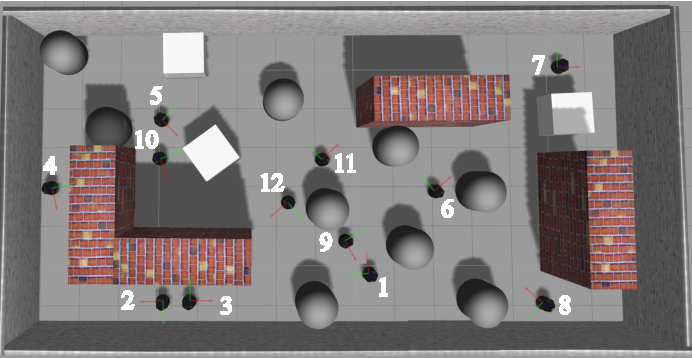
\includegraphics[width=0.8\columnwidth]{figure/obstacle_figs/start_env_number}
    \caption{The simulated indoor environment implemented in \textit{Gazebo} with various scenes and obstacles. The \textit{Turtlebot} is the experimental agent with a \textit{Kinect} camera mounted on it. One of the 12 locations marked in the figure is randomly set as the start point in each  training episode. The red arrow of every location represents the initial moving direction.}
   \label{fig:ob_environment_figure}
\end{figure}
%----------------------------------------------------


In our previous work \cite{tai2016deep}, the training datasets were collected in structured corridor environments. Depth images in these datasets were labelled with real-time moving commands from human decisions. In this chapter, to extend the navigation ability of the mobile robot, we set up a more complex indoor environment, as shown in Fig.~\ref{fig:ob_environment_figure}, in the \textit{Gazebo}\footnote{http://gazebosim.org} simulator. Besides the corridor-like traversable areas, there are much more complicated scenes like cylinders, sharp edges and multiple obstacles with different perceptive depths. These newly created scenes have never been used in the training of our previous supervised learning model \cite{tai2016deep}.

We use a \textit{Turtlebot} as the main agent in the simulated environment. A \textit{Kinect} RGBD camera is mounted on top of the robot. We can receive the real-time RGB-D raw image from the field of view (FOV) of the robot. All of the requested information and communications between agents are achieved through \textit{ROS}\footnote{http://www.ros.org} interfaces.



%----------------------------------------------------
\subsection{Deep Reinforcement Learning Implementation}
%-------------network structure---------------------
   \begin{figure}[!t]
      \centering
      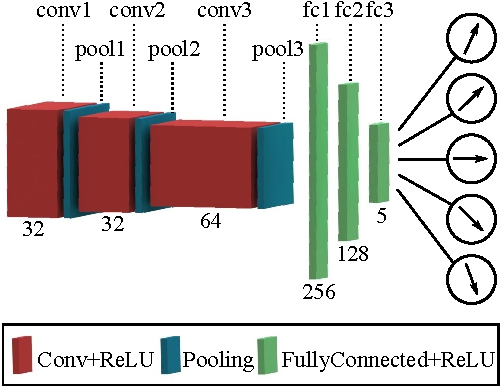
\includegraphics[width=0.75\columnwidth]{figure/obstacle_figs/cnn_structure}
      \caption{The network structure for the actor-evaluation estimation. It is a combination of convolutional networks for feature extraction and fullyconnected layers for policy learning. They have been separately proven to be effective in our previous works \cite{tai2016deep, tl_rcar_2016}.}
      \label{fig:ob_network_structure}
   \end{figure}
%-------------------------------------------------

As a standard reinforcement learning structure, we set the environment mentioned in Section \ref{sec:ob_simuenvi} as $e$. At each discrete time step, the agent selects an action $ a_t $ from the defined action set. In this section, the action set consists of five moving commands, namely \textit{left, half-left, straight, half-right} and \textit{right}. Detailed assignments of speeds related to the moving commands are introduced in Section \ref{sec:ob_experiment}. The only perception by the robot is the depth image $x_t$ taken from the \textit{kinect} camera after every execution of the action. Unlike in Atari games, where the reward $r_t$ is the change of the game's score, the only feedback used as the reward is a binary state, indicating whether a collision occurs or not. This is decided by checking the minimum distance $l_t$ through the depth image taken by the \textit{Kinect} camera. Once a collision occurs, we set a negative reward of $t_{ter}$ to represent the termination. Conversely,
we grant a positive reward of $t_{move}$ to encourage collision-free movement.

The state sequences $s_t$ in the simulated environment are regarded as a \textit{Markov Decision Process} (MDP) which is an alternate combination of moving commands and depth-image states, where $s_t = \{x_1,a_1,x_2,a_2,\dots, a_{t-1},x_t\}$. The sequence terminates once the collision happens. As the assumption of the MDP, $x_{t+1}$ is completely decided by $(x_t, a_t)$ without any reference to the former states or actions in $s_t$. The sum of the future rewards until the termination is $R_t$. With a discount factor $\gamma$ for future rewards, the sum of future estimated rewards is $R_t = \sum_{t'=t}^{T} \gamma^{t'-t} r_{t'}$, where $T$ means the termination time-step. The target of reinforcement learning is to find the optimal strategy $\pi$ for the action decision through maximizing the action-value function $Q^*(x,a) = max_{\pi}\mathbb{E}[R_t|x_t=x,a_t=a,\pi]$.
The essential assumption in DQN \cite{mnih2015human} is the \textit{Bellman equation}, which transfers the target to maximize the value of $r+\gamma Q^{*}(x',a')$ as
\[ Q^{*}(x,a)=\mathbb{E}_{{x'}\sim{e}}[r+\gamma \max \limits_{a'}Q^{*}(x',a')|x,a]. \]
Here, $x'$ is the state after acting action $a$ in state $x$.
DQN estimates the action-value equation by CNN with weights $\theta$, so that $Q(s,a,\theta) \approx Q^{*}(s,a)$.
%----------------------------algorithm-----------------------
\begin{algorithm}[!ht]
    \caption{Deep reinforcement learning algorithm}
    \label{alg:training_al}
    \begin{algorithmic}[1]
    \STATE {Initialize the weights of evaluation networks as $\theta^-$\\
           Initialize the memory $D$ to store experience replay\\
           Set the collision distance threshold $l_s$
           }
    \FOR {episode $ = 1, M$}
    \STATE {Randomly set the \textit{Turtlebot} to a start position\\
            Get the minimum intensity of depth image as $l_t$\\
        \WHILE{$l_t>l_s$}
            \STATE { Capture the depth image $x_t$ }
            \STATE {With probability $\varepsilon$ select a random action $a_t$ \\
                    Otherwise select $ a_t =\mathrm{argmax}_a Q(x_t,a;\theta^-)$ \\}
            \STATE { Move with the selected moving command $a_t$\\
                    Update $l_{t}$ with new depth information\\
            \IF{$l_{t}<l_s$}
                \STATE{ $r_t =r_{ter}$ \\
                $x_{t+1} = Null$}
            \ELSE
                \STATE{ $ r_t = r_{move}$ \\
                Capture the new depth image $ x_{t+1}$}
            \ENDIF \\
            }
            \STATE{
            Store the transition $(x_t,a_t,r_t,x_{t+1})$ in $D$} \\
            Select a batch of transitions  $(x_k, a_k, r_k, x_{k+1})$  randomly from $D$ \\
                \IF {$r_k = r_{ter}  $}
                    \STATE{ $y_k = r_k$   }
                \ELSE
                \STATE{  $ y_k = r_k+\gamma \max_{a'} Q(x_{k+1},a';\theta^-) $ }
                \ENDIF \\
           Update $\theta$ through a gradient descent procedure on the batch of $ (y_k - Q(\phi_k,a_k;\theta^-))^2$
        \ENDWHILE}
    \ENDFOR
\end{algorithmic}
\end{algorithm}
%-------------------------------------------------------

In this section, we use three convolutional layers for feature extractions of the depth image and use an additional three fullyconnected layers for obstacle avoidance learning. The structure is depicted as red and green cubes in Fig.~\ref{fig:network_structure}. To increase the non-linearity for better data fitting, each Convolutional or Fullyconnected layer is followed by a Rectified Linear Unit (ReLU) activation function layer.
The number under each Conv+ReLU or FullyConnected+ReLU cube is the number of channels of the output data related to this cube. The network takes one depth raw image as the input. The five channels of the final fully-connected layer \textit{fc3} are the values of the five moving commands. Also, to avoid the overfitting in the training procedure, both of the first two fully-connected layers \textit{fc1} and \textit{fc2} are followed with a dropout layer. Note that dropout layers are eliminated in the test procedure \cite{srivastava2014dropout}.

Algorithm \ref{alg:training_al} shows the workflow of our revised deep reinforcement learning process. Similar to \cite{mnih2015human}, we use the memory replay method and the $\varepsilon$-greedy training strategy to control the dynamic distribution of training samples. After the initialization of the weights for the convolutional networks shown in Fig.~\ref{fig:network_structure}, we set a distance threshold $l_s$ to check if the \textit{Turtlebot} collides with any obstacles. At the beginning of every episode, the \textit{Turtlebot} is randomly set to a start point among the 12 pre-defined start points shown in Fig.~\ref{fig:ob_environment_figure}.
This extends the randomization of the \textit{Turtlebot} locations from the whole simulation world and keeps the diversity of the data distribution saved in memory replay for training.

For the update of weights $\theta$, $y_k$ is the target for the evaluation network. It is calculated by summing the instant reward and the future expectation estimated by the networks with the former weights, as mentioned before in the \textit{Bellman equation}. If the sampled transition is a collision sample, the evaluation for this $(x_k , a_k)$ pair is directly set as the termination reward $r_{ter}$. Setting the training batch size to be $n$, the loss function is
\[
L({\theta}_i) = \frac{1}{n} \sum_{k}^{n}[(y_k-Q(x_k,a_k;{\theta}_i))^2].
\]
After the estimation of $Q(x_k, a_k)$ and $\max_{a'} Q(x_{k+1},a')$ with the former $\theta^-$, the weights $\theta$ of the network will be updated through back-propagation and stochastic gradient descent.
